\documentclass[12pt]{article}       % 設定文件類型為 article,字體大小為 12pt
\usepackage[T1]{fontenc}            % 設定 T1 字型編碼,確保特殊字元的正確顯示
\usepackage{lmodern}                % 強制使用 Latin Modern 字型,提高可讀性和相容性
\usepackage{fontspec}               % 允許使用 OpenType 和 TrueType 字型
\usepackage{graphicx}               % 支援插入圖片
\usepackage{amsmath}                % 提供數學環境和公式支持
\usepackage{csquotes}               % 提供引用格式支援
\usepackage{comment}                % 提供多行註解


%biber NSTC_project

%=================================================={{{參考文獻設定}}}==================================================

\usepackage[style=ieee, maxnames=99]{biblatex}          % 設定參考文獻格式為 IEEE,最多顯示 99 個作者
\addbibresource{NSTC_project.bib}                       % 添加參考文獻檔案 references.bib
\renewcommand{\bibfont}{\fontspec{Times New Roman}}     % 設定參考文獻字體為 Times New Roman
\renewcommand{\UrlFont}{\fontspec{Times New Roman}}     % 設定 URL 連結字體為 Times New Roman
\DeclareFieldFormat{url}{\url{#1}}                      % 格式化 URL
\bibliography{your_bib_file}                            % 引用你的 .bib 文件

%=================================================={{{目錄設定}}}==================================================

\usepackage{tocloft}                                            % 自訂目錄格式

% 設定目錄的點線填充樣式
\renewcommand{\cftsecleader}{\cftdotfill{\cftdotsep}}           % 節(section)
\renewcommand{\cftsubsecleader}{\cftdotfill{\cftdotsep}}        % 小節(subsection)
\renewcommand{\cftsubsubsecleader}{\cftdotfill{\cftdotsep}}     % 子小節(subsubsection)

% 設定目錄標題格式
\renewcommand{\contentsname}{\centering \LARGE \textbf{目錄}}    % 目錄標題置中,字體大小為 LARGE,加粗

%=================================================={{{字體設定}}}==================================================

% 設定英文字體
\newfontface\englishfont{Times New Roman}               % 自訂英文字體命令 \englishfont,使用 Times New Roman

\setmainfont[
    ItalicFont={Times New Roman Italic},                % 設定斜體
    BoldFont={Times New Roman Bold},                    % 設定粗體
    BoldItalicFont={Times New Roman Bold Italic}        % 設定粗斜體
]{Times New Roman}                                      % 設定主要英文字體為 Times New Roman

% 設定中文字體
\usepackage{xeCJK}                                      % 使用 xeCJK 套件來處理中文
\setCJKmainfont[BoldFont={標楷體-繁}, ItalicFont={標楷體-繁}] {標楷體-繁}

%=================================================={{{版面設定}}}==================================================

% 設定頁面邊界,適用 A4 紙張
\usepackage[top=2cm, bottom=2cm, left=2cm, right=2cm, a4paper]{geometry}

% 設定行距與段落格式
\usepackage{setspace}
\onehalfspacing % 設定 1.5 倍行距
\setlength{\parskip}{6pt} % 設定段落間距 6pt
\setlength{\parindent}{2em} % 設定段落首行縮排 2 個字元

%=============================================================================================================================
%=============================================================================================================================
%=============================================================================================================================

\begin{document}

\pagenumbering{roman}  
\setcounter{page}{1}  % 從 I 開始

%=================================================={{{中文摘要}}}==================================================

\section*{\centering 摘要}  % 只讓標題置中
\addcontentsline{toc}{section}{摘要}  % 手動加入摘要到目錄

%==============================摘要內容==============================

\hspace{2em}
近年來無人機(Unmanned Aerial Vehicle, UAV)整合各種附加設備且隨著飛行控制系統及自動化技術逐漸趨近成熟,
在軍事、執法、科技應用領域不斷蓬勃發展,其中四軸旋翼無人機更具有安全、低成本等優點。
攝影和錄影是無人機其中一項重要功能,因其擁有遠超一般攝影手段的視野角度,並且在空間上受到的環境限制相對較少。
這使得無人機在捕捉廣大場景方面表現出色,遠勝於其他方法所能呈現的效果。
目前中國部分城市已開始運用無人機進行科技執法\cite{chinatimes2019},
台北市與台中市警察局也以成立無人機機隊\cite{cna_2022}\cite{tai_2021},進行交通觀測。
透過無人機提供的視角,執法人員能夠快速監視交通情況。

本研究計畫旨在開發一套智慧交通巡檢系統,以無人機為主要執行工具。
該系統將透過事先建立的資料庫,使無人機能夠有效偵測違停車輛。
與目前固定式照相桿等科技執法裝置相比,無人機具有大範圍監控的優勢,且能夠極大地降低設備成本。
不同於先前方式先判斷紅線再確認車輛是否違規的方法。
本計畫將透過無人機的GPS位置資訊來判斷車輛是否違規停放以避免車輛停放於紅線上或完全遮掩紅線的情形。
由於系統僅針對違規區域進行檢查,因此能有效提升巡邏速度,縮短偵測與回報的時間。
預期的成果是透過設計的電腦應用程式,能夠標示出不可停車的區域,而無人機則透過事先建立的資料庫,
比對飛越指定區域所拍攝的影像,快速偵測違規車輛並記錄其位置,
運用透視變換(Perspective Transformation)與空間對位(Georeferencing)達到對指定區域車輛違停進行有效監控的目標。
此系統優勢在於高效率的監控,更在於能夠大幅減少設備投資成本,同時提升違停車輛檢測的靈活性和即時性。

%==============================摘要內容==============================
\newpage  % 插入換頁命令,將目錄和後續內容分開

%=================================================={{{英文摘要}}}==================================================
\section*{\centering Abstract}  % 只讓標題置中
\addcontentsline{toc}{section}{Abstract}  % 手動加入摘要到目錄
%==============================摘要內容==============================



%==============================摘要內容==============================
\newpage  % 插入換頁命令,將目錄和後續內容分開

%=================================================={{{目錄}}}==================================================

\begin{center}
\tableofcontents  % 插入目錄,並置中
\thispagestyle{empty}  % 讓目錄頁沒有頁碼
\end{center}
\newpage  % 插入換頁命令,將目錄和後續內容分開

%=================================================={{{內容開始}}}==================================================

\pagenumbering{arabic}  % 開始使用阿拉伯數字頁碼
\setcounter{page}{1}  % 設定頁碼從 1 開始

%\englishfont{this is an example of mixed English and Chinese.}

\section{\centering 緒論}
%==============================內文==============================

\subsection{研究背景} 
%==============================內文==============================
\hspace{2em}無人機的應用已在軍事、執法及科技領域取得顯著成效。
尤其在交通監控領域,無人機具有廣闊的視野和較低的環境限制,相較於傳統的固定式監控設備,無人機具備了更高的靈活性和效率。
現有的交通執法裝置,如固定式照相桿,雖然能夠進行監控,但無法提供大範圍的即時監測,且設備成本較高。
隨著無人機技術的進步,無人機在交通巡檢中展現了出色的潛力,尤其在違停車輛的偵測方面,無人機能夠提供更靈活且高效的解決方案。

%==============================內文==============================
git add .		暫存
\subsection{研究動機} 
%==============================內文==============================
\hspace{2em}目前的研究和應用大多針對車輛橫跨紅線進行判斷,但對於完全蓋住紅線或停在紅線與白線交界處的情況,現有方法無法準確判斷車輛是否違停。
因此,本研究計畫的動機在於利用無人機的GPS位置資訊來判斷車輛的違規情形,避免車輛完全遮掩紅線或停在紅線邊界處的情況。
通過建立資料庫並使用無人機拍攝影像,比對車輛所處位置與違規區域,能夠快速偵測違規車輛並進行即時回報,進一步提升交通執法的效率與靈活性。


%==============================內文==============================


\subsection{研究問題} 
%==============================內文==============================
\hspace{2em}


%==============================內文==============================


\section{\centering 文獻探討與回顧}
%==============================內文==============================
\hspace{2em}


%==============================內文==============================


\section{\centering 研究方法及流程}
%==============================內文==============================
\hspace{2em}


%==============================摘要內容==============================


\section{\centering 研究結果}
%==============================摘要內容==============================



%==============================摘要內容==============================


\section{\centering 結論} 
%==============================摘要內容==============================



%==============================摘要內容==============================

\section{\centering 參考文獻}
\vspace{-3.5em}  % 減少與上方內容的間距
\renewcommand{\refname}{}  % 去除 "References" 標題
\printbibliography  % 列出參考文獻
\end{document}

%=============================================================================================================================
%=============================================================================================================================
%=============================================================================================================================


\begin{comment}
    %==============================圖片==============================
    \begin{figure}[h]
        \centering
        \renewcommand{\figurename}{圖} %顯示圖1,不是figureat1
        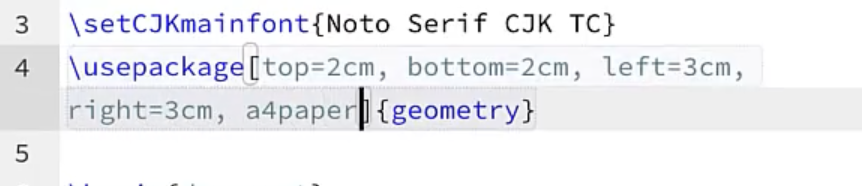
\includegraphics[width=0.5\textwidth]{截圖 2025-01-24 03.21.17.png}     %圖片檔案名稱
        \caption{這是圖片的標題}    %圖片檔案名稱
        \label{fig:example2}    %為圖片添加標籤
        %\ref{fig:example1}
    \end{figure}
    
    %==============================數學公式==============================
    \begin{align}
        a &= b + c \label{eq:1}
        \\
        d &= e - f \label{eq:2}
        %式label{eq:2}
    \end{align}
    
    %==============================表格==============================
    \begin{table}[ht]
        \centering
        \begin{tabular}{|c|c|c|}
        \hline
        項目  & 數量 & 價格 \\
        \hline
        蘋果  & 10  & 30   \\
        香蕉  & 5   & 15   \\
        橙子  & 8   & 20   \\
        \hline
        \end{tabular}
        \caption{水果表格}
        \label{tab:fruits}
    \end{table}
    
    \end{comment}
        